\chapter{Design}\label{design}

The following chapter will expose the design process and reasoning
behind certain design decisions made for the prototypes. It will lead
through the different prototyping stages and user testing to an
evaluation of the design, including an outlook.

The prototyping was happening in three subsequent stages. The first
stage comprised a set of pencil sketches on paper; the second prototype
was created with web technology, but fixed around a certain source code
and faked interactivity; the third prototype was implemented as a
plug-in for the Atom editor, and is able to work with any source code it
is provided.

\section{Definitions}\label{definitions}

To be able to talk about the qualitites of the concept and prototypes,
we must first define a number of terms.

\begin{description}
\item[Scope block]
In a JavaScript text file, a scope block is the textual block
representing a logical scope. For a function, which in JavaScript
creates a new scope, the scope block starts at the \texttt{function}
keyword and ends at the closing curly brace \texttt{\}} of the function
body. If, in a text editor, the cursor is placed anywhere inside this
scope block (but outside of child scopes), the scope block is called
\emph{active scope}.
\item[Current scope]
In a running JavaScript program, it is the currently executed scope.
This is a term related to the run-time rather then to author-time, and
should not be confused with \emph{active scope} described below.
\item[Active scope]
The scope which is currently in focus of editing. In relation to IDEs,
code editors and the prototypes presented in this chapter, the active
scope always describes the scope that the cursor is placed in.
\item[Local scope]
In the context of nested scopes, the local scope is the one in focus (be
it in the execution context during run-time, or the editing context
during author-time). Local scope is contrasted with non-local scope;
scopes that are logically distant from the local scope. Those may be
ancestor scopes, descendant scopes, or parallel scopes. The term is also
used to contrast \emph{global scope}.
\end{description}

\section{Sketching}\label{sketching}

One could argue that sketching is part of the earlier exploration phase,
rather than of the prototyping phase. However, next to sketching
different ideas, the author also sketched different possible
implementation for one feature that seemed valuable to the design
solution: \emph{highlighting}.

The basis for the sketches were printouts of the same source code, each
leading to a different way of highlighting.

(scans here)

\subsubsection{Active scope, inclusive}\label{active-scope-inclusive}

This sketch highlights the active scope block by applying a background
colour to it. The highlighting is \emph{inclusive}, i.e. any descendant
(inner) scopes are highlightes as well.

\subsubsection{Active scope, exclusive}\label{active-scope-exclusive}

Same as above, but descendant scope blocks are excluded from
highlighting. This way of highlighting was implemented in the scripted
prototype (see \ref{}).

\subsubsection{Active scope and ancestor
scopes}\label{active-scope-and-ancestor-scopes}

Next to highlighting the active scope, its ancestor scopes can also be
highlighted to emphasize nesting. To contrast the ancestor scopes from
the active scope, the highlighting would make use of different
background colours, for example different shades of grey. This way of
highlighting can be combined with both the inclusive and exclusive
approach.

\subsubsection{Scope colouring}\label{scope-colouring}

Described by Crockford \citeyear{crockford} as „context colouring“, this
way of highlighting would not apply a background colour, but instead
replace the existing forms of syntax highlighting. Thus, the
highlighting would not depend on the cursor position (which defines the
\emph{active scope}), but would be static instead.

\subsubsection{Identifier origin}\label{identifier-origin}

Additionally to emphasizing code blocks, individual identifiers can be
highlighted. Given a highlighted active scope, this sketch highlights
identifiers that are defined in that scope but used somewhere else (in
descendant scopes).

This works as well for the \emph{scope colouring} described above, as
each scope has a fixed colour. Identifiers that are used in other scopes
than they are defined in can therefore always be recognized if they
appear in the colour of their origin scope.

\section{Scripted prototype}\label{scripted-prototype}

It very quickly became clear that the sketches were of little value.
Although most of them gave a general impression on where the selected
scope started and where it ended, it did not allow the user to see the
big picture. It seemed probably that a more interactive prototype would
be more helpful in this regard. As its capabilities of working with code
are limited and the code had to be specifically prepared, this is called
a \emph{scripted prototype}.

As the author is most familiar with web technologies, the scripted
prototypes would be built using \ac{html}, \ac{css} and JavaScript and
run in a web browser. Other prototyping tools, such as Balsamiq or
Indigo Studio, would not allow for enough detail in terms of
highlighting certain code passages, and would have represented a
learning overhead.

\begin{figure}[htbp]
\centering
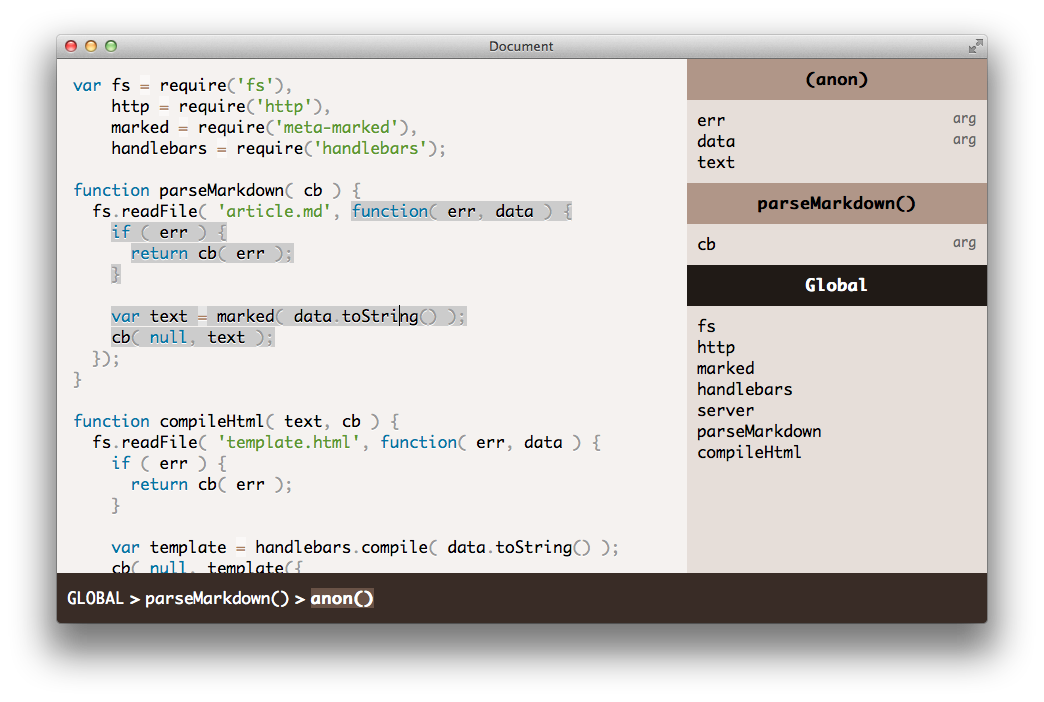
\includegraphics[keepaspectratio,width=0.75\textwidth,height=0.75\textheight]{img/prototype-1.png}
\caption{Screenshot of the scripted prototype run in a browser}
\label{fig:syntaxhighlighting}
\end{figure}

A code syntax highlighter\footnote{Prism, see \url{http://prismjs.com/}}
was used to turn the subject source code into styled \ac{html} tags, to
make it appear as if it was inside of a real code editor. Applying
syntax highlighting was also necessary to see if the different
highlighting techniques, as sketched out in the previous phase, would
interfere with syntax highlighting.

Furthermore, markers in the form of HTML tags were added to the subject
source code, which made it possible to apply different
styles\footenote{For example text colours, background colours, of font styles.}
to regions of the code. This was later used to realize highlighting of
the \glspl{scope-block}.

Two distinct \ac{ui} elements were added: a sidebar and a bottom bar.
The content of both depends on the \emph{active scope}, i.e. the scope
the cursor is placed in.

For each of the nested \ac{scope-block} that the cursor is positioned in
(beginning from the local scope, going outwards up to the global scope),
the sidebar shows a pane. Each pane contains the scope’s name along with
a list of identifiers defined within that scope. In opposition to the
working prototype, the scripted prototype does not show phenomena like
hoisting and shadowing. The panes are ordered ascending by logical
distance, i.e. the local scope would be on top, the next surrounding
scope beneath it, and so forth; up to the global scope on the bottom.

The different panes are hardcoded: all panes exist in the markup of the
prototype at all times and are pre-filled with the relevant data, but
are shown and hidden on demand.

The bottom bar shows a horizontal list of scope names. It makes use of
the \emph{breadcrumbs} \ac{ui}
pattern\footnote{In the Yahoo pattern library: \url{https://developer.yahoo.com/ypatterns/navigation/breadcrumbs.html}}.
Each listed scope, beginning from the global scope on the very left, up
to the local scope on the right, can be highlighted and navigated to by
clicking on its label. By
hovering\footnote{Hovering: Placing the mouse cursor over an element.}
over the label, the user can get a preview of the target scope, as it is
highlighted in the editor alongside the currently active scope.

\subsection{Constraints}\label{constraints}

The scripted prototype has some drawbacks, some of which might influence
its quality. The most obvious one is the fact that it only works with a
static, predefined source code, which is manually adapted to serve the
prototype’s purpose. This implies that

\begin{enumerate}
\def\labelenumi{\arabic{enumi}.}
\itemsep1pt\parskip0pt\parsep0pt
\item
  changes can not be made to the code, which makes the experience of the
  prototype very different from a real code editor, and
\item
  it is hard to tell if the prototype works similarily well with code
  that is more complex, less complex, or of an overall different style.
\end{enumerate}

The fact that there are no text editing facilities comes with another
drawback, namely the absence of a cursor. If a cursor cannot be placed
anywhere in the editor, the „activation“ of a scope block must be
achieved differently. In the case of this prototype, it is solved by
clicking on a piece of code. However, clicking anywhere in the line
besides the actual text will not change the active scope.

\subsection{Evaluation of the scripted
prototype}\label{evaluation-of-the-scripted-prototype}

The prototype was tested with two JavaScript developers in individual
in-person walkthrough sessions. The users were introduced to the
concept, if they were not familiar with it already, and explained the
basic constraints of the prototype (as mentioned above). They were
thereafter able to explore and test the prototype to their likings. One
of the two sessions have been recorded as a screencast.

The users liked both the „preview“ feature (hovering over a breadcrumb)
and the sidebar. The preview gave them an opportunity to quickly get a
visual overview of your position in the code and the active scope chain.
The sidebar showed them which variables and functions are available in a
given context. Overall, they liked the dynamicity of the prototype, as
they could „play around“ with it and understand the design concept just
by trying. They quickly made a connection between they position of the
cursor and the active scope along with its content.

One of the users suggested possible improvements or alternative designs
for existing features. He recommended a wider use of colour coding to
create a link between the scope in the editor window and the sidebar,
for example by colouring all the ancestor scopes in different shades of
grey. He also suggested an alternative visual structure for the sidebar
instead of the list, for example nested clusters or a graph. For
hoisting, the user came up with an idea to integrate indicators into the
text editor: a „phantom“ variable declaration, which would be grey and
not editable, could be inserted on top of a scope, to show that a
certain variable declaration would be hoisted up there. This indicator
should be collapsible so that it does not interfere with the editing
process. Because of technical constraints, this idea was not implemented
in the next prototype iteration; however, it seems a sensible solution
to the hoisting indication problem, as it communicates this implicit
phenomenon very clearly.

In conclusion, the prototype was well-received and served its purpose
well. It became clear that a consistent and clear visual language for
the next iteration of the prototype was necessary, and that a direct
connection between the code and the scope visualization has to be
communicated.

\section{Working prototype}\label{working-prototype}

The second prototype, which emerged into the final one, was built as a
working prototype capable of handling any JavaScript scope, rather than
as a proof-of-concept. It was integrated into the
Atom\footnote{See \url{https://atom.io/}} text editor as a so-called
\emph{package}, released as \gls{oss} and was made publicly available
for using and testing. The package is called „Scope Inspector“ and will
be referred to using this name throughout this section.

\subsection{The prototyping platform}\label{the-prototyping-platform}

For the prototype to yield meaningful results, I decided to integrate it
into a real \ac{ide}. This decision was informed by several
circumstances. The first and most obvious is that I could address a
broader community of users this way. If the prototype was, like the
scripted prototype, implemented in isolation as a standalone
application, it would raise the barrier for people to test and for me to
distribute it. But by building it as a plug-in to an existing \ac{ide},
I could leverage the distribution channels that were already in place. A
second reason is that users are already familiar with the software and
do not have to orientate themselves anew. This also implies that all the
features that the user \emph{expects} from an \ac{ide} are in place, and
the prototype can more seamlessly be integrated into the user’s
workflow. Finally, the third reason for building a prototype on top of
an existing \ac{ide} is that it can make use of the design language in
place, which eliminates the need to take decisions that are rather
irrelevant for this prototype, such as the choice of a typeface and
colour palette.

As a prototyping platform, the author decided on the Atom text editor.
Atom is open source and created by the software company Github. By the
time of writing, Atom is a relatively young project with a growing
community and plug-in ecosystem. The reasons for deciding in favour of
Atom are threefold: the technologies it is built upon, its internal
software architecture, and the user group it is targeting.

Atom is built on web technologies, namely
WebKit\footnote{See \url{http://www.webkit.org/}} and
Node.js\footnote{See \url{http://nodejs.org/}}. WebKit is the browser
engine used by the web browsers Google Chrome and Apple Safari, amongst
others, and is therefore responsible for the \acl{ui} layer of Atom.
Node.js is the JavaScript platform responsible for running any
non-\ac{ui} logic. Atom is mostly written in
CoffeeScript\footnote{CoffeeScript is a programming language that transcompiles to JavaScript.}.
Consequently, Atom packages can be written in CoffeeScript or
JavaScript, using HTML and CSS for the \ac{ui}. As I am familiar with
these technologies, Atom provided an ideal prototyping platform with a
low entry barrier.

For extending Atom, it offers an \ac{api} which can be used by plug-ins.
Atom’s internal architecture is built in a modular way, so that plug-ins
can hook into nearly everything that happens and react on it. The
prototype makes use of this fact in many ways, for example by showing
and hiding its \ac{ui} elements depending on the type of file that is
being edited. In general

Atom is marketed by Github as a „hackable text editor for the 21st
Century“\footnote{See \url{https://atom.io/}, accessed 18.05.2014}. It
is also intended to be a „deeply extensible system that blurs the
distinction between ‚user‘ and ‚developer’.“ Those claims lead to the
conclusion that Atom is a text editor built for developers,
especially—but not exclusively—web developers. While not every web
developer is a proficient JavaScript developer, the target groups of
Atom and this prototype seem to overlap to a large extent.

\subsection{Parsing and gathering relevant
information}\label{parsing-and-gathering-relevant-information}

For the prototype to be as \emph{complete} and \emph{correct} as
possible, it was built on top of an existing JavaScript parser called
Esprima\footnote{See http://esprima.org/}. The process of extracting the
relevant scope structure and annotations from the
\ac{ast}\footnote{The \ac{ast} is the data structure that is returned by the parser, which contains all the lexical statements and expressions.}
will not be discussed here in greater detail, but is instead described
in a blog post \cite{tvo}.

However, it is important to mention what data structures are extracted
from the source code. Analoguous to the nature of JavaScript scope as
described in chapter \fullref{research}, the data structure is a
hierarchy of objects. Each object represents a scope and may have
metadata as well as a list of identifiers attached to it. An identifier
is either a child scope (as created by a function) or a variable. For
scope objects, the metadata are its name and its location in the source
code (row and column of the start and end points), whereas for variables
the metadata are its name, location, if it is hoisted, by which child
scope identifiers it is shadowed, and which identifier it is shadowing.

A diagram of an exemplary data structure is shown in figure
\ref{parser}.

\textbf{TODO: insert diagram of data structure here}

Using this data structure, the prototype can show meaningful data to the
user, which would not have been possible with the \ac{ast} alone. The
modular composition of the prototype, which decouples the task of
parsing from the task of displaying information, makes it possible to
re-use each of the components. The component described in this section,
which is responsible for turning the \ac{ast} into a „scope tree“, could
be used in plug-ins for any \ac{ide} to achieve similar functionality as
the one of this prototype.

\subsection{Interface and
Interactions}\label{interface-and-interactions}

The design respects that the subject of a developer’s work is the code
itself, not the tools that surround it. This is why the solution
integrates into the most important part of the IDE, the text editor,
directly. The features built into the editor itself will be called
\emph{inline} features.

Atom’s interface is, by default, threefold: the text editor takes the
most space; on its left is a sidebar containing a file browser, and on
the bottom is a status bar. As many web browsers, text editors, and
IDEs, multiple open files are accessed through \emph{tabs} on the top of
the screen. The tabs are important, because the Scope Inspector will
only be active as long as an editor with a JavaScript file is in the
foreground. Whenever the user switches to another tab, the Scope
Inspector is activated or deactivated, depending on if the tab contains
an editor with a JavaScript file or not.

Throughout the Scope Inspector package, a visual style consistent with
Atom’s is used. Any icons in use are taken from the
Octicons\footnote{See \url{https://github.com/styleguide/css/7.0}} icon
set, which is incorporated into every Github product. Atom supports
themes (colour schemes) for both the application window and the editor.
Scope Inspector makes use of the colours defined in those themes. This
way, the package \ac{ui} feels more natural to the user. However, there
may be difficulties if the theme is not well-defined and the colours are
badly balanced. One user reported very low contrast between the editor’s
background and the scope highlighting. In addition to pre-defined theme
colours, Atom also provides a set of pre-styled \ac{ui} components, for
example buttons and panes, which have been used in the prototype.

Whenever the Scope Inspector is active, two things are obvious: on the
bottom of the editor, a panel is shown which we call \emph{bottom bar},
and the active scope is highlighted inline. Additionally, a sidebar can
be toggled using the Atom command „Scope Inspector: Toggle Sidebar“.
This command is accessible using the menu, the command palette, a
keyboard shortcut (\texttt{Ctrl+Alt+i} by default), and a toggle button
on the bottom bar. The several components and their functionality are
explained in more detail in the following sections.

\subsubsection{Inline scope
highlighting}\label{inline-scope-highlighting}

As explained above, the \emph{active scope} is the immediate scope the
cursor is placed in. It is emphasized by highlighting it through a
lighter or darker background colour (depending on Atom’s colour scheme).
If the cursor is placed in a different scope, the formerly active scope
is un-highlighted, and the now active scope is highlighted instead.

While the scripted prototype implements \emph{exclusive highlighting},
this prototype now implements \emph{inclusive highlighting}, which means
that the inner scope are highlighted as well. This is due to technical
reasons; building exclusive highlighting into the prototype would have
taked a lot more time. In further iterations of the prototype, an option
to enable and disable exclusive highlighting could be provided.

The bottom bar contains a toggle
button\footnote{A switch in the form of a button, which can be either *on* or *off*.}
to enable or disable highlighting of the global scope. Highlighting the
global scope with \emph{inclusive highlighting} is not useful, as the
whole file would be highlighted (and there would be nothing left to
contrast the highlight to).

\subsubsection{Bottom bar}\label{bottom-bar}

The bottom bar serves two purposes: it provides a quick glance of where
in the scope hierarchy the cursor is and provides quick access to two
settings.

On the right side of the bottom bar, to toggle buttons allow for
enabling and disabling of two features. The right button, showing a list
icon, shows or hides the sidebar. The left button with the label
„Highlight Global“ toggles the highlighting of the global scope (as
described above).

The left side of the bottom bar shows the breadcrumbs known from the
scripted prototype. The breadcrumbs, implemented as simple buttons, are
labeled with the corresponding scope name. The global scope is always on
the left, whereas the currently local, active scope is on the right. By
hovering over any of the breadcrumb buttons, the user can preview the
respective scope highlighting in the editor. The preview is applied in
addition to the currently active highlight in a different colour.

By hovering over the breadcrumbs from left to right or from right to
left, the user can make the relationship between the logical structure
of the JavaScript program (in the form of hierarchic scopes) and the
textual structure (in the form of code) visible.

\subsubsection{Sidebar}\label{sidebar}

The sidebar shows content depending on the currently active scope.
Similarily to the scripted prototype, the sidebar lists one pane for
each scope in the hierarchy of the active scope. The active scope is
listed on top, while its ancestors are listed below, up to the global
scope on the very bottom.

Each pane is entitled by the name of the scope. In case of function
scope, the name of the function becomes the scope name („(anonymous
function)“ in the case of an unnamed function expression). In case of
the global scope, the name is „GLOBAL“.

Underneath the title, the names of all identifiers defined within the
scope are listed, along with certain attribute annotations.

\begin{itemize}
\itemsep1pt\parskip0pt\parsep0pt
\item
  Function parameters are listed first. They appear with the annotation
  „param“, set in smaller text size to the right.
\item
  General variables follow the parameters. If they are not shadowed,
  they have no annotations.
\item
  Functions are the last entities in the list. They are connotated with
  a pair of parantheses „()“.
\end{itemize}

The listed identifiers show also if they are hoisted, shadowed, or if
they shadow other identifiers. This is indicated by different stylistic
changes.

\begin{itemize}
\itemsep1pt\parskip0pt\parsep0pt
\item
  Hoisted identifiers have a small, upwards-pointed arrow on the left
  side of their label. This indicates that their declaration is
  implicility moved upwards in code.
\item
  Shadowed identifiers are printed in a more subtle text colour. Besides
  that, their label is striked-through to indicate that they are not
  accessible within the given descendant scope.
\item
  Identifiers that shadow other identifiers in ancestor scopes are
  printed in a highlight colour. In case of Atom’s standard \ac{ui}
  theme, this is a bright blue colour.
\end{itemize}

\section{User Testing \& Evaluation}\label{user-testing-evaluation}

The goal of user testing was to collect both qualitative and
quantitative data through different methods. The quantitative data
collection was built into the prototype in form of a connection with
Google Analytics\footnote{A website and app analytics platform.}.

\subsection{Test installment}\label{test-installment}

Atom includes a package management system with an online repository,
called \ac{apm}. This system allows any developer to publish Atom
packages and thus make them available for any Atom user to download and
use. Consequently, this prototype was distributed via \ac{apm}.

The author was collaborating with two full-time developers and one
part-time developer. They agreed to install the package and use it over
the course of one week (full-time developers) or one day (part-time
developer), respectively, integrating it into their usual workflows.

\begin{itemize}
\itemsep1pt\parskip0pt\parsep0pt
\item
  2 inquiries
\item
  hintergrund der thesis erklären
\item
  klar machen dass dev weiß wie scope funzt
\end{itemize}

In addition to this directed user test, publishing the prototype via
\ac{apm} made it available to the general public. It was announced on
several social networks, especially targeting existing Atom users, with
the goal of getting users to download and use it. A week after
publishing the prototype, the number of downloads counted ???. This way
of testing „in the wild“ makes it harder to gather feedback, compared to
the method of addressing potential users directly. However, the
analytics mechanism built into the prototype yielded quantitative data
for evaluation.

\subsection{Usage metrics}\label{usage-metrics}

The prototype was built with the option to collect usage metrics using
the Google Analytics service. By default, this option was set to
\emph{off}, as I oppose the unknown tracking of any data for ethical
reasons. However, users were asked in the \texttt{README} file, which is
displayed both on the package’s
page\footnote{See \url{https://atom.io/packages/scope-inspector}} and on
Github\footnote{See \url{https://github.com/tvooo/scope-inspector}}, to
enable tracking in Atom’s \emph{settings} panel for the Scope Inspector
package.

If enabled, the following events are tracked:

\begin{itemize}
\itemsep1pt\parskip0pt\parsep0pt
\item
  The package is enabled/disabled
\item
  The sidebar is shown/hidden
\item
  The user hovers over a scope breadcrumb in the bottom bar and thus
  previews a scope highlighting
\item
  The user clicks on a scope breadcrumb in the bottom bar and thus jumps
  to the beginning of scope, making it the active scope and highlighting
  it
\end{itemize}

Through collecting these events, a claim can be made—to a certain
extent—for how helpful certain features are.

\subsection{Testing Results}\label{testing-results}

\subsubsection{Analytics}\label{analytics}

Analytical metrics have been tracked over the course of 13 days. In
total, five different users (including myself) had tracking enabled,
with a peak of fours simultaneous users. On average, two to three users
contributed data each day.

In those nearly two weeks, the sidebar was enabled 76 times, whereas
interactions with elements on the bottom bar happened 144 times.
However, only 22 of those interactions were clicks which have to happen
intentionally—the hover events can occur by chance (for example by
moving the mouse from the editor window to the status bar and
vice-versa). Given those circumstances, it can be concluded that the
sidebar was more in use than the bottom bar. But event metrics can not
measure if users used the bottom bar for orientation, for example just
by looking at it and figuring out where in the scope hierarchy they are.
Thus, the analytics result are of limited use for the evaluation of the
prototype.

\subsubsection{Interviews with
developers}\label{interviews-with-developers}

This section summarizes the finding of the user testing, as collected
through interviews. None of the interviewees had used the prototype
before, and both are only casual Atom users.

\begin{description}
\itemsep1pt\parskip0pt\parsep0pt
\item[(Inline) Hoisting Indicator]
None of the developers discovered the inline hoisting indicator. One of
them did not know the concept of hoisting, while another one
misinterpreted the indicators (upwards arrows) in the sidebar. He
assumed that they are pointing upwards because clicking on them would
cause the editor to scroll upwards, navigating to the identifier’s
declaration.
\end{description}

\begin{itemize}
\item
  hoisting war unbekannt
\item
  inline hoisting-anzeige hat niemand gesehen, musste gezeigt werden
\end{itemize}

\begin{description}
\item[Sidebar]
One functionality that each user found to be missing was a means of
navigation through the sidebar. Two users expected to be able to jump to
a variable declaration if he sees a problem there, just by clicking on
the variable’s name. Another user thought the ability to scroll to a
certain variable was denoted by the upwards pointing arrow next to it.
It was also suggested to be able to jump to the beginning of a scope by
clicking on its respective headline, similar to what happens when the
user clicks a breadcrumb in the bottom bar. Adding line numbers for each
identifiers was also suggested, in order to be able to distinguish
anonymous functions better from each other.

The order of the panels, each representing one scope in the scope chain,
was confusing to some users. Although they understood the concept of a
scope chain, they expected it to be in the order that scopes appear in
code. However, code is linear, while scope is hierarchical, and they do
not map directly. It is reasonable to assume that the order which is
used in the prototype is learnable for the users, as it works
analogously to \ac{css} in the Chrome DevTools. This could for example
be achieved by connecting the scope in the sidebar visually with its
counterpart in the editor. One user suggested that, when a scope is
hovered in the sidebar, its counterpart in the editor could be
highlighted (analogous to the effect of hovering a breadcrumb in the
bottom bar).

Another suggestions concerning the sidebar was to highlight even single
variables in the editor when they are highlighted in the sidebar.
Regarding shadowing, one user was able to detect a bad practice in his
code during testing: he had created a shadowing situation in which the
two variables of the same name server completely different purposes.
\item[Bottom bar]
None of the users discovered on their own the possibility to navigate
the scope chain by clicking on the breadcrumbs. However, after pointing
the feature out, they stated it was useful. One user noted that, once
you navigate into a higher scope, you can not go „back“ to the last
position (or the previously selected scope, which is nested inside the
now active scope).

Two users stated that the bottom bar would take up too much space, as
most developers would like as much space as possible for their code.
They suggested to style the breadcrumbs more like hyperlinks on the web,
and also to indicate that they are breadcrumbs by deparating them
through rightwards pointed arrows. One user even suggested to get rid of
the bottom bar completely, in case that the sidebar would take its tasks
of navigating and previewing the scope chain.
\item[Modularity]
One of the users asked if he could disable the inline highlighting
altogether, as he could imagine it to be annoying in the long run; this
is not possible in the final prototype, as during the design phase the
highlighting was considered a central element of the design. He
suggested that all three parts of the prototype—inline highlighting,
sidebar, and bottom bar—should be optional.
\item[Miscellaneous]
bla
\end{description}

\begin{itemize}
\item
  Was ist mit einem überblick: zeige mir mal schnell alle shadowings und
  hoistings in einer datei. wird beides vom linter nicht erkannt, ist
  aber code smell.
\item
  bug entdeckt: function innerhalb von array wird nicht erkannt, was
  z.B. bei der asnyc library vorkommt
\item
  gleichzeitiges highlighten: wenn ich in bottom bar hover, wird
  gleichzeitig im code UND in der sidebar gehighlightet, und vice versa
\item
  er selber hat fast nie probleme mit dem scope, hat sich angewöhnt
  variablen klar zu deklarieren etc
\item
  ich sollte mich mehr auf die performance-geschichte konzentrieren
\item
  intelligente warnungen, „best practices“ einbauen. man sieht zwar was
  angezeigt wird, aber was bedeutet das?
\item
  bisschen direkter, ne warning oder so
\item
  ne whitelist oder so
\item
  performance-argument ist interessant, sollte man mehr einbauen. was
  haben sachen für nen impact auf performance?
\item
  man muss wissen, wie man es deuten kann
\item
  „ist schon fast zu viel für das was es tut“ -\textgreater{} closures
  anzeigen hat auch nen lerneffekt, für anfänger etc, aber sogar
  advanced devs wissen nicht immer was da geht
\end{itemize}

i used it for a day but it never realy gave me any benefits, the code
was to well writen, i think

\begin{itemize}
\itemsep1pt\parskip0pt\parsep0pt
\item
  i dont think i did understand everything
\item
  but also, the code i was working on wasnt that complicated
\item
  but it was not inthe way
\end{itemize}

zusammenfassend\ldots{}

\begin{itemize}
\itemsep1pt\parskip0pt\parsep0pt
\item
  sidebar am nützlichsten, eine gewisse übersicht, eine sicht auf den
  code, wenn man damit noch navigieren könnte wäre doll
\end{itemize}

\subsubsection{Social Media Feedback}\label{social-media-feedback}

In the open source software community, social media channels are
frequently used to state an opinion on new products, to share news, and
to give feedback. The prototype, in the form of the Scope Inspector
package for Atom, received some positive feedback on different channels.

On Twitter, which was used as a marketing instrument as well, the
feedback was exclusively positive. One user called it „another reason to
consider switching from {[}Sublime Text to
Atom{]}“\footnote{See \url{https://twitter.com/adardesign/status/466589449561055232}},
while others seemed to be interested as
well\footnote{See \url{https://twitter.com/raganwald/status/466930480517246976}}.
Five tweets mentioning the package have been both retweeted and
favourited about 20
times\footnote{Based on tweets that could be found by the Twitter search for the keyword ```scope inspector’’’.}.

On the news platforms EchoJS and Reddit (JavaScript section) the package
got little attention: four and eight upvotes, respectively, although the
only comment on Reddit claims that it „looks
promising“\footnote{See \url{http://www.reddit.com/r/javascript/comments/25k30l/javascript_scope_inspector_an_atom_package_to/chi27cm}}.

On Github, users filed two issues (bugs). One user requested the
possibility to investigate identifiers in the sidebar more deeply (which
is impossible to do correctly if the program is not executed). The other
one asked for on-the-fly re-evaluation of the scope, as was already
asked for in the interviews. At the stage of the prototype, scope is
only re-evaluated when the file is saved; however, looking at linting
tools, re-evaluating a short time (100-200ms) after the user stopped
typing seems to be a promising
strategy\footnote{See \url{https://github.com/tvooo/scope-inspector/issues/7}}.
This method would have been tested in terms of performance.

Several
reactions\footnote{See \url{http://www.echojs.com/comment/9867/1} and \url{https://twitter.com/vilmosioo/status/466934333681717248}}
on the blog post about the technical side of the Scope Inspector
\cite{tvo} suggest that there are difficulties for JavaScript developers
to deal with CoffeeScript code. In other words, the target users of the
package (JavaScript developers) are not directly able to improve on or
modify the package itself. This complicates code contribution for this
open source project.
